\ifdefined\COMPLETE
\else
\documentclass[12pt]{article}

\usepackage{algorithm}
\usepackage{mathtools,amsmath,amssymb,amstext,amsthm,tikz,thmtools}
\usepackage[inline]{enumitem}

\usepackage[utf8]{inputenc} % allow utf-8 input
\usepackage[T1]{fontenc}    % use 8-bit T1 fonts
\usepackage{hyperref}       % hyperlinks
\usepackage{url}            % simple URL typesetting
\usepackage{booktabs}       % professional-quality tables
\usepackage{amsfonts}       % blackboard math symbols
\usepackage{nicefrac}       % compact symbols for 1/2, etc.
\usepackage{microtype}      % microtypography

\newcommand{\mc}{\mathcal}
\newcommand{\mb}{\mathbf}
\newcommand{\tr}{\text{Tr}}
\newcommand{\diag}{\text{diag}}
\newcommand\numberthis{\addtocounter{equation}{1}\tag{\theequation}}

\DeclareMathOperator*{\argmin}{arg\,min}
\DeclareMathOperator*{\argmax}{arg\,max}

\newtheorem{theorem}{Theorem}
\newtheorem{lemma}[theorem]{Lemma}
\newtheorem{definition}[theorem]{Definition}
\newtheorem{proposition}[theorem]{Proposition}
\newtheorem{corollary}[theorem]{Corollary}

\begin{document}
\fi

\section{Introduction}
Clustering aims to group similar data instances together while separating dissimilar ones. However, often many datasets have, on top of cohesive groups, a subset of ``unstructured'' points as well. In such cases, the goal is to detect the cohesive structure while simultaneously separating the unstructured data points. Clustering in such situations can be viewed as a {\em noise-robustness} problem. 

Another important issue is that the clustering problem is {\em under-specified}. This means that the same dataset might need to be clustered in different ways depending upon the intended application. Consider, for example, the problem of clustering users of a movie-streaming service such as Netflix. The output clustering can be used to suggest similar movies to similar users or to gain insights into the daily/monthly behaviour of the users. Depending on the application, different clustering algorithms need to be chosen. Hence, any solution to clustering challenges like noise-robustness, under-specificity should be such that it is applicable across a wide-range of clustering algorithms. 

We propose a general method of regularisation that transforms any clustering objective which outputs $k$ clusters to one that outputs $k+1$ clusters. The algorithm is now allowed to `discard' a bunch of points into the extra `garbage' or noise cluster by paying a constant regularization penalty. The intuition is that this will make it easier to detect the structure in the remaining points. Similar to regularisation, {\em noise prototypes} (points which are equidistant to all other points) were considered by \cite{dave1993robust}. However, that idea was used only in the limited context of Lloyd’s algorithm and without any theoretical or noise robustness guarantees.

In this paper, we consider the following framework motivated by \cite{ben2014clustering}. We are given an input dataset $\mc X$ made of two components. The first is the clusterable or ``nice'' subset $\mc I$ which is the union of $k$ unit balls $B_i$ separated by a distance of atleast $\delta$. The second is the unstructured noise component $\mc N$. Note that the clustering algorithm only sees $\mc X$ and is not aware in advance of $\mc I$ or $\mc N$. The addition of $\mc N$ makes it more difficult to detect the structure in $\mc I$. Consider the original algorithm $\mc A$ and its robustified transformation $\mc A' = \mc R_{\lambda}(\mc A)$. $\mc A'$ is obtained by using our regularisation paradigm and specifying a parameter $\lambda$. By comparing the clusterings $\mc A(\mc I)$ and the clustering $\mc A'(\mc X)$ restricted to $\mc I$, we can examine the effect of $\mc N$ (in terms of size and distance relative to $\mc I$) on the ability to detect the cohesive structure of $\mc I$.

In this work, we consider two choices for $\mc A$. An algorithm based on SDP relaxation of the $k$-means objective and another based on LP relaxation. \cite{awasthi2015relax} showed that for $\delta > 2\sqrt{2}(1+\frac{1}{\sqrt d})$ (where $d$ is the dimension of the euclidean space) the SDP-based algorithm recovers the clustering of $\mc I$ if the balls $B_i$ are generated by an isotropic distribution (stochastic ball model). \cite{iguchi2015tightness} `improved' this to $\delta > 2 + \frac{k^2}{d}cond(\mc I)$. However, the condition number (ratio of maximum distance between any two centers and the minimum distance between any two cluster centers) can be arbitrarily large. We improve this to $\delta > 2\big(1+\sqrt\frac{k}{d}\big)$ which is optimal for large $d$. To our knowledge, this is best known guarantee for the SDP-based $k$-means algorithm. Note that all the above results are for the noiseless case. For the noisy case, our robustified (or regularised) version recovers the clustering of $\mc I$ for $\delta > 2\big(1+\sqrt{\sigma + \frac{k}{d}}\big)$ where $\sigma$ is a term which depends on the ratio of number of noisy points and the number of points in the smallest cluster. 

We also consider the distribution-free setting where  the balls $B_i$ have been generated by any unknown distribution. In this setting, the separation requirement for recovering the structure of $\mc I$ becomes $\delta > 2(1 + \sqrt{k})$ for the noiseless and $\delta > 2(1+\sqrt{\sigma + k})$ for the noisy case. As before, $\sigma$ depends on the number of noisy points. We also give robustness guarantees for the LP based algorithm. However, the separation requirement in this case is more strict $\delta > 4$ and the requirements on noise are also stronger (noisy points from the set $\mc N$ should be far from $\mc I$).  

We also prove hardness results for the regularised $k$-means objective. For $k \ge 2$, the NP-hardness follows from the NP-Hardness of the standard (non-regularised) $k$-means objective. We show that the regularised objective is NP-Hard to optimize even for $k=1$. An important choice in the implementation of the regularised algorithm is the value of the regularization constant $\lambda$. For $\lambda = 0$, the problem becomes trivial and for $\lambda \rightarrow \infty$, the problem reduces to $k$-means. We prove that there exists a range of $\lambda$ depending on the sizes of the clusters and the separation $\delta$ between them such that the regularised algorithm recovers the underlying structure when given that $\lambda$ as input. We also conduct simulation studies where we examine the effect of $\lambda$, the number of noisy points $m$, the separation $\delta$ and other parameters on the performance of our regularised SDP-based algorithm. We also perform experiments on the MNIST dataset. We observed that the regularised version performed better than $k$-means++ when the dataset had outliers. In the absence of outliers, the performance of both these algorithms were similar. 

\subsection{Related Work}
The problem of clustering in the presence of noise has been studied before both in distribution-based and distribution-free settings. In the distribution-based setting, the goal is to estimate the parameters of the distribution (say the mean and variance of gaussian etc). In the distribution-free setting, the goal is to prove that if the data has some structure (is clusterable) then the (proposed or existing) clustering algorithm recovers that structure even in the presence of noise. Different works define different notions of `clusterable' data. In the current work, the separation requirement on the clusters was global. That is, the each cluster was separated by atleast $\delta$ times the maximum radius amongst all the clusters. Other notions of clusterability, like $\alpha$-center proximity \cite{awasthi2012center}or $\gamma$-margin \cite{ashtiani2016clustering} require that two clusters be separated relative to their radii.

Different works on clustering have also made different assumptions on the type of noisy points. The most common is to assume that the noise is adversarial but the number of adversaries is not too large. For example, \cite{balcan2012clustering} and \cite{balcan2008discriminative} provide bounds for clustering in the presence of noise as long as the number of adversaries is constant-factor smaller compared to the size of the smallest cluster. \cite{kushagra2016finding} considered noise which is structureless, that is the noisy points do not form dense large subsets. Another field of work is to address noisy part of the data as being generated by some uniform random noise or gaussian perturbations \cite{cuesta1997trimmed}, \cite{garcia2008general} and \cite{dave1993robust}.  

Another line of work which is related to ours is clustering a mixture of $k$ gaussians with few adversaries. The best known result is by \cite{awasthi2012improved} which requires that the mean of the gaussians be separated by $\tilde O(\sigma \sqrt{k})$ where $\sigma^2$ is an upper bound on the variance of the $k$ gaussians. Recently, \cite{charikar2017learning} matched this result using different techniques. Although the distribution free setting considered in this paper is different from the above works, the separation required for the SDP-based algorithm to succeed also has a similar dependence on $k$, namely $\delta > 2(1 + \sqrt{k})$. 

Some works examine the robustness of different algorithms when the number of clusters is the same for the original data and the data with added noise. They show that in this setting the traditional algorithms are provably not noise-robust \cite{hennig2008dissolution} and \cite{ackerman2013clustering}. Another line of work which is related to ours is based on the convex relaxation of center-based clustering objectives. \cite{peng2007approximating} was the first to formulate the $k$-means cost function as a 0-1 SDP and then subsequently relaxed it to a standard SDP. In this work, we use a similar technique to first obtain a 0-1 SDP and subsequently a relaxed SDP for the regularised $k$-means objective. 

\section{Preliminaries and definition}
\label{sec:pre}

Let $(\mb M, d)$ be a metric space. Given a finite set $\mc X \subset \mb M$, a $k$-clustering $\mc C$ of $\mc X$ partitions the set into $k$ disjoint subsets $\mc C = \{C_1, \ldots, C_k\}$. An objective-based clustering algorithm associates a cost with each possible partition of $\mc X$ and then tries to find the clustering with minimum cost. Throughout this section, $f$ denotes a function on the nonnegative reals.

\begin{definition}[$(k, f)$-objective algorithm] Given $\mc X\subset \mb M$ and a distance function $d$, a $(k, f)$-objective based algorithm $\mc A$ tries to find centers $\mu_1, \ldots, \mu_k \in \mb M$ so as to minimize the following function
\begin{align}
\label{eqn:kfObjectiveAlg}
\text{Cost}(\mu_1, \ldots, \mu_k) = \sum_{x\in \mc X} f(d(x, \mu(x))), \quad \mu(x) = \argmin_{\mu \in \{\mu_1, \ldots, \mu_k\}} d(x, \mu).
\end{align}
\end{definition}
Note that algorithm $\mc A$ may not often find the optimal solution because for many common functions $f$, solving the optimization is NP-Hard. Thus, heuristics are used that can get stuck at a local minima. For example, when $f(x) = x^2$, the above definition corresponds to the $k$-means objective, and the Lloyd's algorithm that is used to solve this objective can get stuck at a local minima. 

\begin{definition}[$(k, f)$-$\lambda$-regularised objective algorithm] Given $\mc X\subset \mb M$ and a distance function $d$, a $(k, f)$-$\lambda$-regularised objective based algorithm $\mc A'$ tries to find centers $\mu_1, \ldots, \mu_k \in \mb M$ and set $\mc I\subseteq \mc X$ so as to minimize the following function
\begin{align}
\label{eqn:kfObjectiveAlg}
\text{Cost}(\mu_1, \ldots, \mu_k, \mc I) = \sum_{x\in \mc I} f(d(x, \mu(x))) + \lambda |\mc X \setminus \mc I|,
\end{align}
where $\mu(x) = \argmin_{\mu_i} d(x, \mu_i).$
\end{definition}

The regularised objective allows discarding certain points into a ``garbage'' cluster at the expense of paying a constant penalty. The intuition is that this will help the algorithm better detect the structure of the remaining points. We will see in \S \ref{section:hardness} that minimizing this objective function is NP-Hard for all $k \ge 1$.

\subsection{Robustification paradigms}
\begin{definition}[$\lambda$-Regularised Paradigm] The $\lambda$-regularised paradigm is a robustification paradigm which takes as input a $(k, f)$-objective algorithm $\mc A$ and returns a $(k, f)$-$\lambda$-regularised objective algorithm $\mc A'$.  
\end{definition}

In this work, we focus on robustification of the $k$-means objective. Hence, it is useful to define the regularised $k$-means objective as we will refer to it many times in the remainder of the paper. 

\subsection{Regularised $k$-means objective}
Given a finite set $\mc X \subset \mb R^{d}$ and an integer $k$, the regularised $k$-means objective aims to partition the data into $k+1$ clusters $\mc C = \{C_1, \ldots, C_{k}, C_{k+1}\}$ so as to solve 
% Changed to put min in objective; seems clearer to me -Nicole
\begin{align}
	\min_{C_1,\ldots, C_{k+1} \atop c_1, \ldots, c_k} \sum_{i=1}^k \sum_{x \in C_i} \|x-c_i\|_2^2 + \lambda |C_{k+1}|.
	\label{eqn:modifiedkmeans}
\end{align}

Note that the first term of the objective depends on the $l_2$ norm, while the second term depends only on the cardinality of the ``noise'' cluster. In order to make our objective function invariant to scaling, the regularization constant $\lambda$ is added to the cost function. 

Let $m(\mc X) := \min_{x\ne y \in \mc X} \|x-y\|_2^2$ and $N = |\mc X|$. Then, it is easy to see when $\lambda \leq \frac{m(\mc X)}{2}$, then \eqref{eqn:modifiedkmeans} admits a trivial solution: each cluster $C_i$ for $i \leq k$ has exactly one point and all the remaining points are in $C_{k+1}$, leading to an objective $\lambda (N-k)$. Indeed, for any other clustering with $|C_i| = n_i$ its objective is at least $\sum_{i=1}^k (n_i-1) m(\mc X)/2 + \lambda n_{k+1} = (n-n_{k+1} - k) m(\mc X)/2 + \lambda n_{k+1}$, where we have used the simple fact:
\begin{align}
\forall C \subset \mc X, ~~
\min_{c} \sum_{x \in C} \|x - c\|_2^2 ~=~ \frac{1}{2|C|}\sum_{x, y \in C} \|x - y\|_2^2.
\end{align}
Comparing the objectives we see the solution is indeed trivial when $\lambda \leq m(\mc X) /2$. Surprisingly, for the interesting case when $\lambda > m(\mc X) /2$, the problem suddenly becomes NP-Hard, as we prove below.

\subsection{Robustness measure}
Given two clusterings $\mc C$ and $\mc C'$ of the same set $\mc X$, we define the distance between them, $\Delta(\mc C, \mc C')$, as the fraction of pairs of points which are clustered differently in $\mc C$ than in $\mc C'$. % I changed this sentence because it didn't make sense -- is this equivalent to what you meant?. -Nicole
Given $\mc I \subseteq \mc X$, $\mc C|\mc I$ denotes the restriction of the clustering $\mc C$ to the set $\mc I$.

\begin{definition}[$\gamma$-robust \cite{ben2014clustering}]
Given $\mc X\subset \mb M$ and clustering algorithm $\mc A$, let $\mc A'$ be its robustified version obtained using any robustification paradigm. Given $\mc I \subseteq \mc X$, we say that $\mc I$ is $\gamma$-robust w.r.t $\mc X \setminus \mc I$ and $\mc A'$ if 
\begin{align}
\Delta(\mc A'(\mc X)|\mc I, \mc A(\mc I)) \le \gamma
\end{align}
\end{definition}
This measure tries to quantify the difference in the clustering of the set $\mc I$ after the addition of `noisy' points $\mc X \setminus \mc I$. If $\mc A'$ is indeed robust to noisy points, then the clusterings should be similar. 



\section{Hardness of regularised $k$-means}
\label{section:hardness}

In this section, we present hardness results for the regularised $k$-means objective. 
%Before we discuss the hardness results, it is worthwhile to mention the trivial case when $\lambda = 0$. In this case the optimization problem is easy and corresponds to the trivial solution of putting every point in the noise cluster $C_{k+1}$. 
The proof for $k \ge 2$ is fairly straightforward and follows from known hardness results for the standard (non-regularised) $k$-means. The more interesting case is when $k = 1$. It is well-known that $1$-means can be solved in linear time \cite{Bellman73} hence the same reduction does not work any more. We reduce an instance of the MAX-CLIQUE problem to the regularised $1$-means problem. We give a proof sketch for the reader's intuition. The technical details can be found in the supplementary section.

%\begin{restatable}{theorem}{hardForAvgdist}\label{lemma:hardForAvgdist}
%Given a clustering instance $\mc X \subset \mb R^d$ and $k \ge 2$, finding the optimal solution to the regularised $k$-means objective is NP-Hard for $\lambda > 0 $.
%\end{restatable}
%\begin{proof}[Proof sketch]
%The idea is as follows. We first show that for a ``big enough'' $\lambda$, the problem is NP-Hard. This is because for a sufficiently large value of $\lambda$, any optimal solution of regularised $k$-means will set $C_{k+1} = \emptyset$, in which case regularised $k$-means reduces to $k$-means, which is known to be NP-Hard \cite{dasgupta2008hardness}. Next, using a scaling argument we show that if the problem is NP-Hard for one $\lambda$, then it is NP-Hard for all $\lambda > 0$.  
%\end{proof}

\begin{restatable}{theorem}{hardForkone}
\label{theorem:hardFork1}
Given a clustering instance $\mc X \subset \mb R^d$. Finding the optimal solution to the regularised $1$-means objective is NP-Hard for all $\lambda > m(\mc X)/2$, where recall that $m(\mc X) := \min_{x\ne y \in \mc X} \|x-y\|_2^2$.
\end{restatable}

\begin{proof}[Proof sketch]
The proof has two parts. We first show that for fixed $\lambda$ the problem is NP-Hard. The proof works by reducing an instance of MAX-CLIQUE to the regularised $1$-mean instance. The idea is to define the distance between any pair of vertices as $1$ if there exists an edge between them. If not, then define the distance as $1 + \Delta$ for a suitably chosen $\Delta$. This construction guarentees that the problem is NP-Hard for atleast one $\lambda > \frac{m(\mc X)}{2}$. Next, using a scaling argument we show that if the problem is NP-Hard for one particular $\lambda$, then it is NP-Hard for all $\lambda > \frac{m(\mc X)}{2}$.
\end{proof}

The above theorem infact shows that regularised $k$-means is hard for all $k \ge 1$. This is becuase we can reduce an instance of regularised $1$-means to regularised $k$-means by placing $k-1$ points very far away. 

\section{The regularised $k$-means SDP-based algorithm}
\label{section:heuristic}
In the previous section, we showed that the regularised $k$-means objective is NP-Hard to optimize. Hence, we cannot hope to solve the problem exactly unless $P=NP$. In this section, we develop an algorithm based on semi-definite programming relaxation of the regularised objective. 

\cite{peng2007approximating} developed an algorithm $\mc A$ (Alg. \ref{alg:heuristicSDP} with $\lambda = \infty$) which tries to minimize the $k$-means objective. They obtained a convex relaxation of the $k$-means objective and solved it polynomially using standard solvers. In this section, we use the same technique to obtain and efficiently solve the convex relaxation of the regularised $k$-means objective. Our algorithm $\mc A'$ (Alg. \ref{alg:heuristicSDP}) is the robustified version of $\mc A$ using the $\lambda$-regularised paradigm. In \S \ref{subsection:sdpAlg}, we give the details of how we transform the regularised objective into an SDP. \S \ref{subsection:sdpRobust} has our main results where we give robustness guarentees for $\mc A'$.    

\begin{algorithm}[t]
\caption{SDP-based regularised $k$-means algorithm}
\label{alg:heuristicSDP}
	\textbf{Input: }{ $\mc{X} \subset R^d$, $k$, and hyperparameter $\lambda$.} \\
	\textbf{Output: }{$\mc C' := \{C_1, \ldots, C_k, C_{k+1}$\}.}
	
	Compute the matrix $D_{ij} = \|x_i-x_j\|^2_2$.\\
	Solve the SDP (Eqn. \ref{eqn:regularisedSDP}) using any standard SDP solver and obtain matrix $Z$ and vector $y$.\\
	Use the rounding procedure (Alg. \ref{alg:roundSDP}) to obtain the partition $\mc C'$. 
\end{algorithm}

 
\subsection{The SDP-based algorithm}
\label{subsection:sdpAlg}
The SDP relaxation of the regularised $k$-means objective is obtained in two steps. Using similar technique to that of \cite{peng2007approximating}, we translate Eqn. \ref{eqn:modifiedkmeans} into a 0-1 SDP (Eqn. \ref{eqn:regularisedSDP}). We then prove that solving the 0-1 SDP exactly is equivalent to solving the regularised $k$-means problem exactly. Then, we relax some of the constraints of the 0-1 SDP to obtain a tractable SDP which we then solve using standard solvers. We then describe the rounding procedure which uses the solution of the SDP to construct a clustering of the original dataset. 

\begin{equation*}
	\begin{split}
	\textbf{0-1}\\
	\textbf{SDP}
  \end{split}
	\begin{cases}
		\min_{Z, y} \enspace &\tr(DZ) + \lambda \langle \mb 1, y\rangle\\
		\text{s.t. } \enspace &\tr(Z) = k\\
		& Z\cdot \mb 1 + y = \mb 1\\	
		&Z\ge 0, Z^2 = Z, Z^T = Z \\
		& y \in \{0, 1\}^n
	\end{cases}
	\xrightarrow{\text{relaxed}} \textbf{ SDP } 
	\begin{cases}
		\min_{Z, y} \enspace &\tr(DZ) + \lambda \langle \mb 1, y\rangle\\
        \text{s.t. } \enspace &\tr(Z) = k\\
		& \Big(\frac{Z+Z^T}{2}\Big)\cdot \mb 1 + y = \mb 1\\		
		&Z \ge 0, y \ge 0, Z \succeq 0 \numberthis\label{eqn:regularisedSDP}
	\end{cases}
\end{equation*}

\begin{restatable}{theorem}{modifiedkmeans}
\label{thm:modifiedkmeans}
Finding a solution to the 0-1 SDP (\ref{eqn:regularisedSDP}) is equivalent to finding a solution to the regularised $k$-means objective (\ref{eqn:modifiedkmeans}). 
\end{restatable}

Equation \ref{eqn:regularisedSDP} shows our 0-1 SDP formulation. The optimization is NP-Hard as it is equivalent to the regularised $k$-means objective. Hence, we consider a convex relaxation of the same. First, we replace $Z^2 = Z$ with $Z \succeq 0$. In addition, we relax $y \in \{0, 1\}^n$ to $y \geq 0$, as the constraint $y\leq 1$ is redundant. Using these relaxations, we obtain the SDP formulation for our objective function.

We solve the SDP using standard solvers \cite{yang2015sdpnal+} thereby obtaining $Z, y$. 
The proof of Thm. \ref{thm:modifiedkmeans} showed that the optimal solution of 0-1 SDP is of the following form. $Z$ is a $n\times n$ block diagonal matrix of the form $\diag(Z_{I_1}, \ldots, Z_{I_k}, 0)$, where $n = |\mc X|$ and $Z_{I_i} = \frac{1}{|C_i|}11^T$. Thus, given $Z$, we can extract the set of cluster centers $C = ZX$ which is an $n \times d$ matrix. Each row $C_i$ contains the cluster center to which data point $x_i$ belongs. For the points $x_j$ assigned to the noise cluster, the corresponding row $C_j$ is zero and $y_j = 1$. The SDP solver does not always return the optimal solution, as the relaxation is not exact. However, we expect that it returns a near-optimal solution. Hence, given $Z$ and $y$ returned by the solver, we use Alg. \ref{alg:roundSDP} to extract a clustering of our original dataset. The $threshold$ parameter indicates our confidence that a given point is noise. In our experiments, we have used a threshold of $0.5$. We did not tune the threshold as in our experiments the results
are not very sensitive to it.

\begin{algorithm}[t]
\caption{Regularised $k$-means rounding procedure}
\label{alg:roundSDP}
	\textbf{Input: }{ $Z \subset \mathbb{R}^{n\times n}$, $y \subset \mathbb{R}^{n}$, $\mc{X}$, and $threshold \in [0,1]$.}\\
	\textbf{Output: }{$\mc C'$.}
	
	If $y_i > threshold$ then
	\begin{itemize}[nolistsep] 
		\item[] Delete $z_i$ and $z_i^T$ from $Z$. Put $x_i$ in $C_{k+1}$.
		\item[] Delete $x_i$ from $X$.
	\end{itemize}
	$k$-cluster the columns of $X^TZ$ to obtain clusters $C_1, \ldots, C_k$.\\
	Output $\mc C' = \{C_1, \ldots, C_k, C_{k+1}\}$.
\end{algorithm}

\subsection{Robustness guarantees}
\label{subsection:sdpRobust}

Assume that we are given a set $\mc I$ of $k$ well-separated balls in $\mb R^d$. That is, $\mc I := \cup_{i=1}^k B_i$ where each $B_i$ is a ball of radius at most one and centered at $\mu_i$ such that $\|\mu_i - \mu_j\| \ge \delta$. On top of this structure, points are added from the set $\mc N$. Let $\mc A$ and $\mc A'$ be the SDP based standard and regularised $k$-means algorithm respectively (as defined in the begining of \S \ref{section:heuristic}). We will show that $\mc I$ is $0$-robust w.r.t $\mc A'$ and $\mc N$ under certain conditions on $\delta$ and mildness properties of the set $\mc N$. To show this, we need to compare the clusterings $\mc A(\mc I)$ and $\mc A'(\mc X)|_{\mc I}$. We first prove recovery guarentees for $\mc A$ in the absense of noisy points.

\begin{theorem}
\label{thm:SDPGeneral}
Given a clustering instance $\mc I \subset \mb R^{N\times d}$ and $k$. Let $\mc I := \cup_{i=1}^k B_i$ where $B_i$ is a finite set of radius at most one centered at $\mu_i$ and $\|\mu_i - \mu_j\| > \delta$. Let $\mc I' = \cup_i B_i'$ where $B_i' := \{x - \mu_i : x \in B_i\}$. Define $ n := \min_{i\in[k]} |B_i|$ and $\rho = \frac{N}{nk}$.
\begin{enumerate}[leftmargin=*,nolistsep,noitemsep]
	\item \textbf{Distribution-free} - If the distance between the centers of any two balls 
$$\delta > 1 + \sqrt{1+ 2\frac{\sigma_{\max}^2(\mc I')}{n}}$$ 
then the $k$-means SDP finds the intended cluster solution  $\mc C^* = \{B_1, \ldots, B_k\}$.
	\item \textbf{Stochastic ball assumption} - Let $\mc P$ denote the isotropic distribution on the unit ball centered at origin. Given points $c_1, \ldots, c_k$ such that $\|c_i - c_j\| > \delta  > 2$. Let $\mc P_i$ be the measure $\mc P$ translated with respect to the center $c_i$. If each $B_i$ is drawn i.i.d w.r.t the distribution $\mc P_i$ and 
$$\delta > 1 + \sqrt{1+\frac{2\theta\rho k}{d}\Big(1+\frac{1}{\log N}\Big)^2}$$  
where $\theta = \mb E[\|x_{pi}-c_p\|^2] < 1$, then there exists a constant $c > 0$ such that with probability at least $1 - 2d\exp(\frac{-cN\theta}{d\log^2N})$ the $k$-means SDP finds the intended cluster solution  $\mc C^* = \{B_1, \ldots, B_k\}$.
\end{enumerate}
\end{theorem}

Thm. \ref{thm:SDPGeneral} improves the result of Thm. 11 in \cite{awasthi2015relax}. Under the stochastic ball assumption, they showed that the $k$-means SDP finds the intended solution for $\delta > 2\sqrt{2}(1+\frac{1}{\sqrt{d}})$. For $k \ll d$, which is the case in many situations our bounds are optimal in terms of the separation reqirement of the clusters.  \cite{iguchi2015tightness} obtained similar results but for $\delta > 2 + \frac{k^2}{d}cond(\mc I)$. Asymptotically, as $d$ goes to $\infty$ their bound matches our result. However, the condition number (ratio of maximum distance between any two centers to the minimum distance between any two centers) can be arbitrarily large. We also have a better dependence on $k$ and $d$. 

Next, we analyse the recovery guarentees for $\mc A'$ in the presence of noisy points $\mc N$. We decompose the noisy points into two disjoint sets $\mc N_1$ and $\mc N_2$. The set $\mc N_2$ consists of all the points which are far from any of the points in $\mc I$. The set $\mc N_1$ consists of points which are close to atleast one of the clusters. We also require that any point in $\mc N_1$ has an $\alpha$-margin w.r.t to the centers of the balls $B_1, \ldots, B_k$. That is the difference of the distance between any point in $\mc N_1$ to a cluster center is atleast $\alpha$. Now, we will show that if $\mc N$ has the aforementioned properties then $\mc I$ is robust w.r.t the regularised SDP algorithm $\mc A'$.

\begin{theorem}
\label{thm:regularisedSDPGeneral}
Given a clustering instance $\mc X \subset \mb R^{N \times d}$ and $k$. Let $\mc X : = \mc I \cup \mc N$. Let $\mc I := \cup_{i=1}^k B_i$ where $B_i$ is a ball of radius at most one centered at $\mu_i$ and $\|\mu_i - \mu_j\| > \delta$. Let $\mc I' = \cup_i B_i'$ where $B_i' := \{x - \mu_i : x \in B_i\}$.  Let $\mc N = \mc N_1 \cup \mc N_2$ have the following properties. For all $p \in \mc N_1$ and for all $i, j$, we have that $| \|p- \mu_i\| - \|p- \mu_j\|| \ge \alpha$. For all $p \in \mc N_2$ and for all $x \in I, \|p - x\| \ge 2\delta$. Note that $\mc N_1 \cap \mc N_2 = \phi$. Let $n = \min_i |B_i|$ and $\epsilon = \frac{|\mc N_1|}{n}$. If $\frac{|\mc N_2|}{n} \le \frac{\delta^2(1-4\epsilon^2)-2\delta(1+4\epsilon)}{\lambda}$ and 
\begin{enumerate}[leftmargin=*,nolistsep,noitemsep]
	\item \textbf{Distribution free} - If  the distance between the centers of any two balls
	\begin{align*}
		\delta > 2 + \frac{9\epsilon}{1-4\epsilon^2} + \sqrt{\frac{2\sigma_{\max}^2(I')}{n(1-4\epsilon^2)}} \text{ and }
		\alpha \ge \sqrt{10\delta \epsilon + 4\delta^2 \epsilon^2+ \frac{2\sigma_{\max}^2(|I'|)}{n(1-4\epsilon^2)}}
	\end{align*} 
	then the regularised $k$-means SDP finds the intended cluster solution  $\mc C^* = \{C_1, \ldots, C_k, \mc N_2\}$ where $B_i \subseteq C_i$ when given $\mc X$ and $\delta^2+2\delta \ge \lambda \ge (\delta-1)^2 + 1$ as input.
	\item  \textbf{Stochastic ball assumption} - Let $\mc P$ denote the isotropic distribution on the unit ball centered at origin. Given centers $c_1, \ldots, c_k$ such that $\|c_i - c_j\| > \delta > 2$. Let $\mc P_i$ be the measure $\mc P$ translated with respect to the center $c_i$. If each $B_i$ is drawn i.i.d w.r.t the distribution $\mc P_i$ 
	\begin{align*}
	   \delta > 2 + \frac{9\epsilon}{1-4\epsilon^2} + \sqrt{\frac{2\rho k\theta(1+\frac{1}{\log|I|})^2}{d(1-4\epsilon^2)}} \text{ and }
	  \alpha \ge \sqrt{10\delta \epsilon + 4\delta^2 \epsilon^2+ \frac{2\rho k\theta(1+\frac{1}{\log|I|})^2}{d(1-4\epsilon^2)}}
	\end{align*}
	then there exists a constant $c_2 > 0$ such that with probability at least $1 - 2d\exp(\frac{-c_2|I|\theta}{d\log^2|I|})$ the regularised $k$-means SDP finds the intended cluster solution  $\mc C^* = \{C_1, \ldots, C_k, \mc N_2\}$ where $B_i \subseteq C_i$ when given $\mc X$ and $\delta^2+2\delta \ge \lambda \ge (\delta-1)^2 + 1$ as input.
\end{enumerate}
\end{theorem}

The proof of both the Thms. \ref{thm:SDPGeneral} and \ref{thm:regularisedSDPGeneral} use the following ideas. We construct a dual for the SDP. We then show that when the conditions of our theorems are satisfied then there exists a feasible solution for the dual program. Moreover, the objective function value of primal and dual sdp program are the same. Hence, the solution found is indeed optimal. The same idea was also used in the proof of Thm. 11 in \cite{awasthi2015relax}. However, our analysis is tighter which helps us to obtain better bounds. The details are in the supplementary section.

We have also developed a regularised version of the $k$-means LP based algorithm. However, due to space constraints we could not include it in the main version of the paper. However, the details and the robustness guarentees for the LP based algorithm are in the appendix. 

\section{Experiments}
We ran several experiments to analyse the performance of our regularised $k$-means algorithm. The first set of experiements were simulations done on synthetic data. The second set of experiments were done on real world datasets like MNIST where we compared the performance of our algorithm against other popular clustering algorithms like $k$-means++. All our experiments were run on Matlab. We solved the SDP formulation using the Matlab SDPNAL+ package \cite{yang2015sdpnal+}. To run $k$-means++ we used the standard implementation of the algorithm available on Matlab.

\subsection{Simulation studies}
The goal of these sets of experiments was to understand the effect of different parameters on the performance of the regularised SDP algorithm. Given the number of clusters $k$, the separation between the clusters $\delta$, the dimension of the space $d$, the number of points in each cluster $n$ and the number of noisy points $m$. We generate a clustering instance $\mc X$ in $\mb R^d$ as follows. We first pick $k$ seed points $\mu_1, \ldots, \mu_k$ such that each of these points are separated by atleast $\delta$. Next we generate $n$ points in the unit ball centered at each of the $\mu_i's$. Finally we add $m$ points uniformly at random. 

We analyse the performance of the regularised SDP algorithm as the parameters change. The most crucial amongst them is the separation between the clusters $\delta$, the regularization constant $\lambda$ and the dimension $d$. Fig. \ref{figure:simulation} shows the heatmap under different parameter values. For each setting of the parameters, we generated 50 random clustering instances. We then calculated the fraction of times the regularised sdp was able to recover the true clustering of the data. If the fraction is close to one, then its color on the plot is light. Darker colors represent values close to zero.

We see an interesting transition for $\lambda$. When $\lambda$ is `too small' then the probability of recovering the true clustering is also low. As $\lambda$ increases the probability of success goes up which are represented by the light colors. However, if we increase $\lambda$ to a very high value then the success probability again goes down. This shows that there is a `right' range of $\lambda$ as was also predicted by our theoretical analysis. 

Another parameter of interest is the dimension of the space $d$. Note that from our theoretical analysis, we know that both the probability of success and the separation depend on $d$. Fig. \ref{figure:simulation} shows that for very low dimension, the regularised sdp fails to perfectly recover the underlying clustering. However, as the dimension grows so does the probability of success. For these two simulations, we fixed the number of points per cluster $n = 30$, $k = 8$ and the number of noisy points $m = 30$. We have similar plots for $(\delta, n)$ and $(\delta, k)$ and $(\delta, m)$ and $(n, m)$. These plots very mostly light colored as long as the number of noisy points was not too large ($\frac{m}{n} \le 5$). Hence, due to space constraints, we have included them only in the supplementary section.
   
\begin{figure}[t]
  \label{figure:simulation}
  \centering
  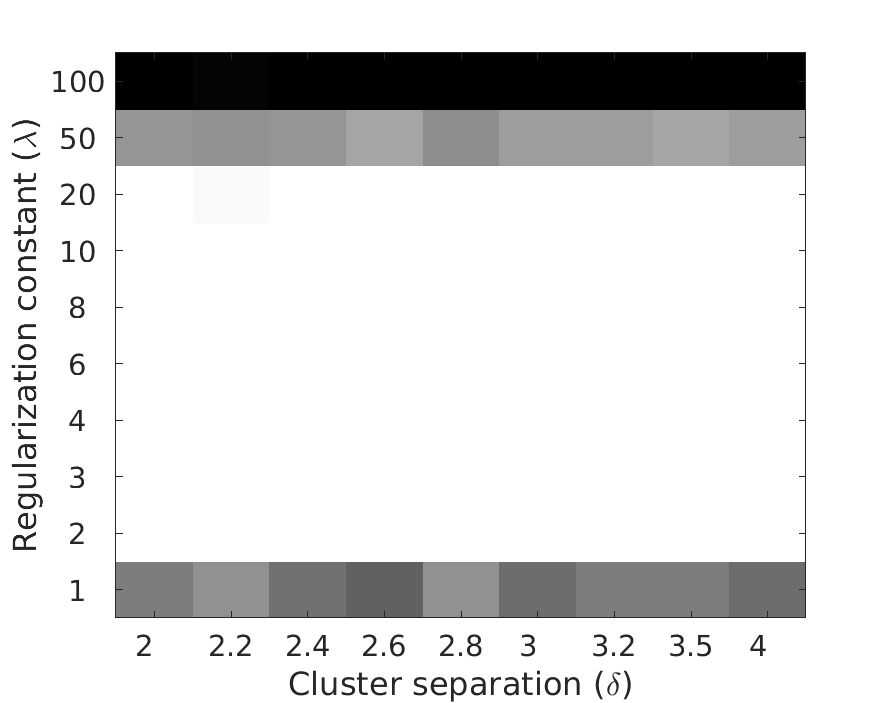
\includegraphics[width=0.4\textwidth]{figures/optimizationClustering/deltaLambda.png}
  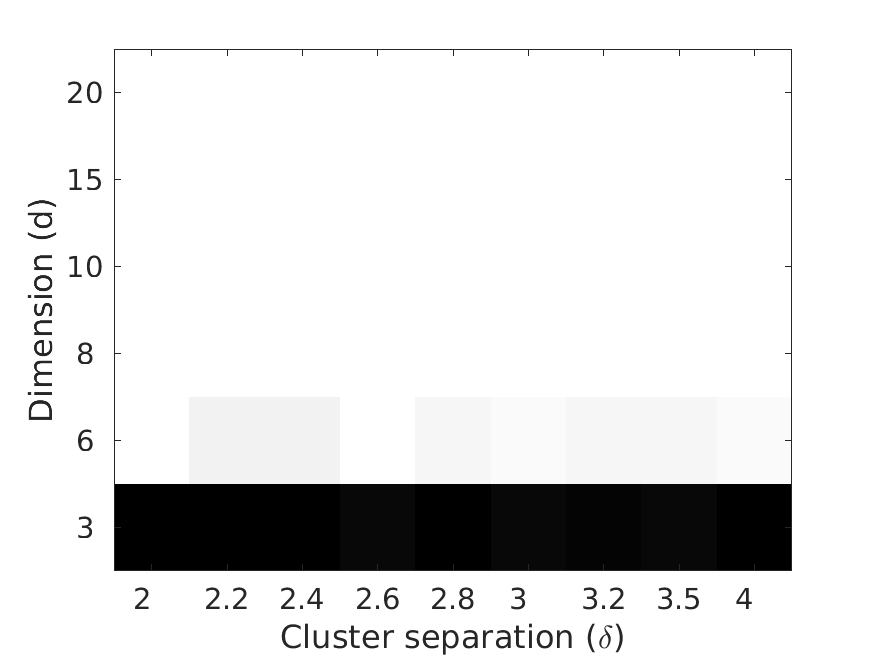
\includegraphics[width=0.4\textwidth]{figures/optimizationClustering/deltaD.png}
  \caption{Heatmap showing the probability of success of the $k$-means regularised sdp algorithm. Lighter color indicates probability closer to one while darker indicates probability closer to zero.}  
\end{figure}

\subsection{Results on MNIST dataset}
We compare our regularised SDP algorithm against $k$-means++ on the MNIST dataset. MNIST is a dataset of images of handwritten digits from zero to nine. It contains 60,000 training images and 10,000 test images. We choose $k = 4$ different classes and randomly sample a total of $N = 1,000$ images from these classes.  We then run both our regularised SDP algorithm and the $k$-means++ algorithm on this dataset. We repeat this process for 10 different random samples of MNIST. We measure the performance of the two algorithms in terms of the precision and recall over the pairs of points in the same cluster. Given a clustering $\mc C$ and some target clustering $C^*$. Define the precision $p$ of $\mc C$ as the fraction of pairs that were in the same cluster according to $\mc C^*$ given that they were in the same cluster according to $\mc C$. The recall $r$ of $\mc C$ is the fraction of pairs that were in the same clustering according to $\mc C$ given that they were in the same cluster according to $\mc C^*$. We finally measure the $f_1$ score of the clustering $\mc C$ as the harmonic mean of its precision and recall. $f_1 = \frac{2pr}{p+r}$. 

Note that the regularised algorithm outputs $k+1$ clusters. Hence, to make a fair comparison, we finally assign each point in the noisy cluster ($C_{k+1}$) to one of the clusters $C_1, \ldots, C_k$ depending upon the distance of the point to the clusters. Another point is that the $f_1$ measures are sensitive to the choice of the $k$ digits or classes. For some choice of $k$ classes, the $f_1$ measures for both the algorithms are higher than compared to other classes. This shows that some classes are more difficult to cluster than other classes. Hence, we only report the difference in performance of the two algorithms. 

We report the performance on datasets with and without noisy points. The first is when there are no outliers or noisy points. In this case, the difference in the $f_1$ values was about $4.34\%$ in favor of $k$-means++. We then added noisy points to the dataset. In the first case, we added images from different datasets like EMNIST (images of handwritten letters). In this case, the difference was $2.54\%$ in favor of the regularised algorithm. In the second case, besides images from different datasets, we also added a few random noisy points to the MNIST dataset. In this case, the difference increased further to about $6.9\%$ in favor of the regularised algorithm. 

\section{Conclusion}
We introduced a regularisation paradigm which can transform any center-based clustering objective to one that is more robust to the addition of noisy points.  We proved that regularised objective is NP-Hard for common cost functions like $k$-means. We then obtained regularised versions of an existing clustering algorithm based on convex (sdp) relaxation of the $k$-means cost. We then proved noise robustness guarentees for the regularised algorithm. The proof improved existing bounds (in terms of cluster separation) for sdp-based standard (non-regularised) $k$-means algorithm. Our experiments showed that regularised sdp-based $k$-means performed better than existing algorithms like $k$-means++ on MNIST especially in the presence of noisy points.
 

\ifdefined\COMPLETE
\else
\end{document}
\fi

